\begin{tikzpicture}
	\fill[pattern=north east lines] (-3,0) rectangle (3,.3);
	\begin{scope}[thick]
	\draw(-3,0)--(3,0);
	
	\path (-2.5,-2.4) node[circle,draw,inner sep=.3cm] (L){}
	(2.5,-1) node[circle,draw,inner sep=.3cm] (R){}
	(0,-3) node[circle,draw,inner sep=.153cm,label=below:$m$] (M){};
	\draw (L.north) -- (L.north|-0,0) (R.north) -- (R.north|-0,0);
	\draw[dashed] (M) -- (0,-1)coordinate (M1);
	\draw (M)  -- (tangent cs:node=L,point={(M.center)},solution=1) coordinate (L1)
	let \p1=($(L1)-(L.center)$),\n1={atan2(\y1,\x1)},\n2={veclen(\y1,\x1)} in
	arc(\n1:180:\n2) -- ++(0,-1.5) node[below,draw]{$m_1$};
	\draw (M)  -- (tangent cs:node=R,point={(M.center)},solution=2) coordinate (R1)
	let \p1=($(R1)-(R.center)$),\n1={atan2(\y1,\x1)},\n2={veclen(\y1,\x1)} in
	arc(\n1:00:\n2) -- ++(0,-1.5) node[below,draw]{$m_2$};
	\end{scope}
	\path pic [draw,angle radius=0.5cm,"$\alpha$",angle eccentricity=1.5] {angle = M1--M--L1} 
	pic [draw,angle radius=0.7cm,"$\beta$",angle eccentricity=1.5] {angle = R1--M--M1} ;
\end{tikzpicture}

\begin{tikzpicture}[>=Latex]
	\draw[thick] (0,0) circle (10mm);
	\draw[thick,->](-1,0)--++(0,-2)node[below]{$T_2$};
	\draw[thick,->](1,0)--++(0,-2)node[below]{$T_2$};
	\draw[thick,->](0,0)--++(0,2)node[above]{$T_1$};
\end{tikzpicture}

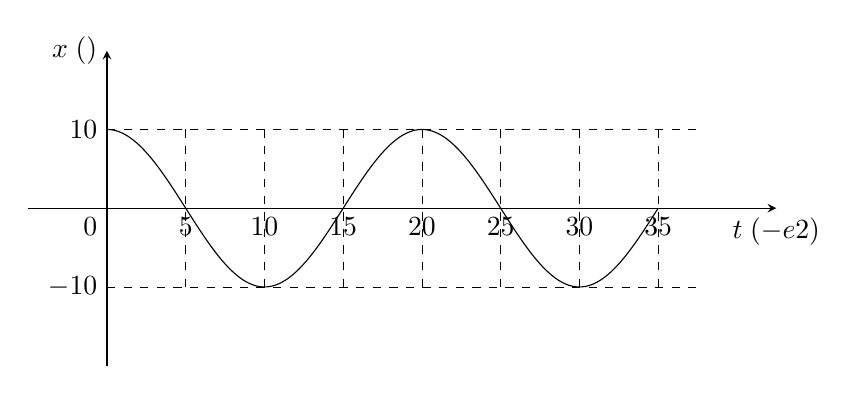
\begin{tikzpicture}[>=stealth]
	\draw[dashed,very thin] (0,-1) grid (7.5,1);
	\draw[->] (0,-2)--(0,2) node[left] {$x\;(\si{\centi\metre})$};
	\draw[->] (-1,0)--(8.5,0) node[below] {$t\;(\SI{-e2}{\second})$};
	\draw plot[smooth,samples=500,domain=0:7] (\x,{cos(deg(pi*\x/2))});
	\foreach \i in {5,10,...,35} \draw (\i/5,0) node[below] {$\i$};
	\draw (0,0) node[below left] {$0$} (0,-1) node[left] {$-10$} (0,1) node[left] {$10$};
\end{tikzpicture}